\documentclass[border=10pt]{standalone}

\usepackage{tikz}
\usepackage{tikzsymbols}
\usetikzlibrary{calc,patterns,shapes.geometric}

\def\centerarc[#1](#2)(#3:#4:#5){\draw[#1] ($(#2)+({#5*cos(#3)},{#5*sin(#3)})$) arc (#3:#4:#5);}

\begin{document}
	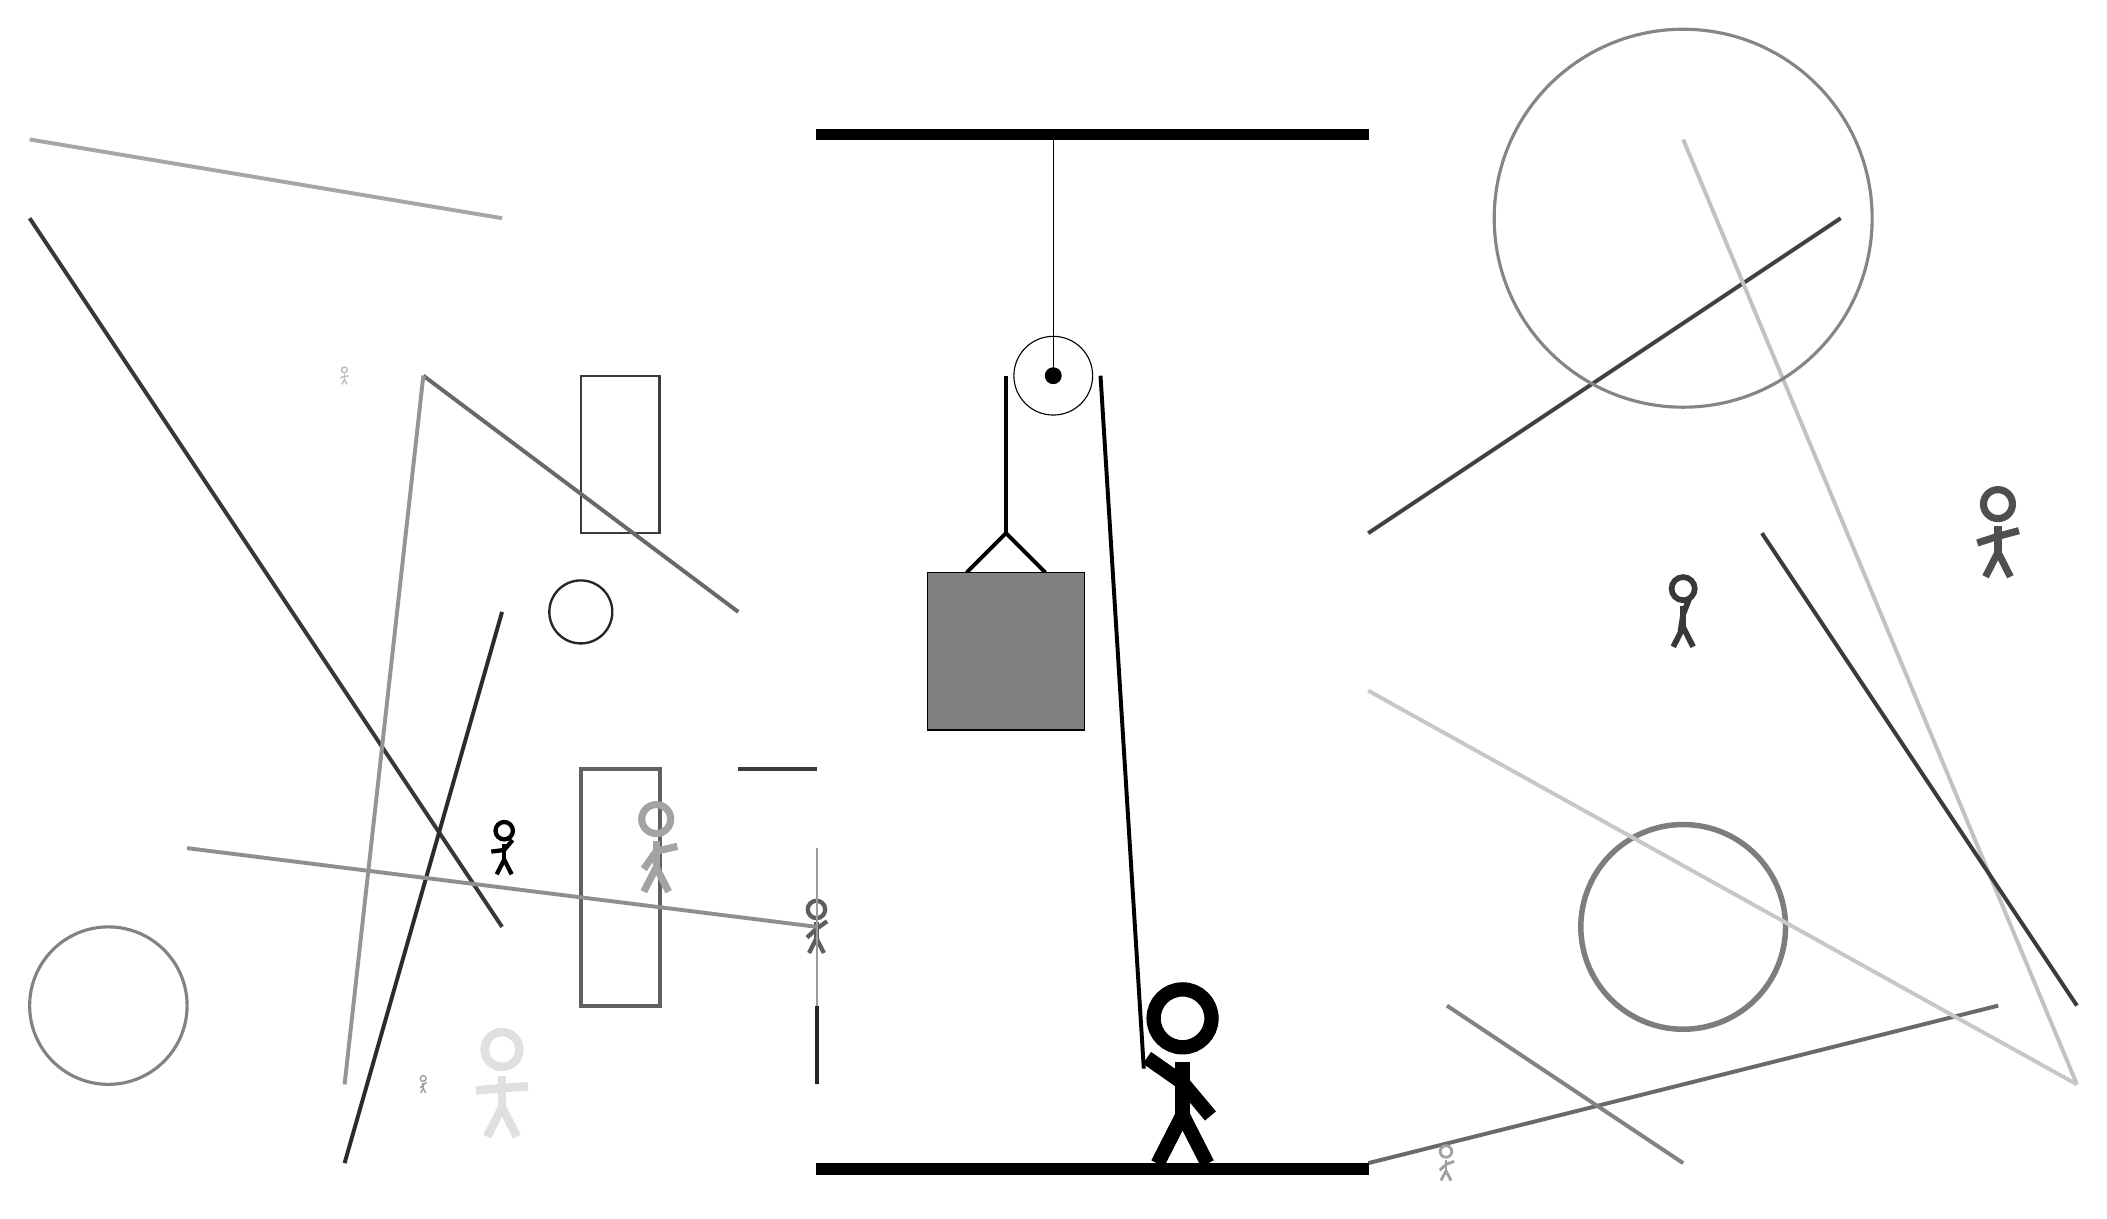
\begin{tikzpicture}
		%%%%% START %%%%%
		
		\draw[fill=black] (-2, 10) rectangle (5, 10.125);
		
		\draw (1, 7) circle (0.5);
		\draw[fill=black] (1, 7) circle (0.1);
		\draw (1, 10) -- (1, 7);
		
		\draw[line width=0.5mm] (-0.1, 4.5) -- (0.4, 5.0) -- (0.9, 4.5);
		\draw[fill=black!50] (-0.6, 4.5) rectangle (1.4, 2.5);
		
		\draw[line width=0.5mm, color=black!74](5, 5) -- (11, 9);
		
		\node[line width=0.5mm, color=black!69] at (13, 5) {\Strichmaxerl[5][18][15]};
		\draw[line width=0.5mm, color=black!62] (-4, -1) rectangle (-5, 2);
		\draw[line width=0.5mm, color=black!59](5, -3) -- (13, -1);
		\draw[line width=0.5mm, color=black!24](9, 10) -- (14, -2);
		
		\node[line width=0.2mm, color=black!26] at (-8, 7) {\Strichmaxerl[1][23][5]};
		\draw[line width=0.3mm, color=black!77] (-4, 7) rectangle (-5, 5);
		
		\draw [line width=0.7mm, color=black!51](9, 0) circle (1.3);
		\draw[line width=0.5mm, color=black!78](-6, 0) -- (-12, 9);
		\draw[line width=0.5mm, color=black!22](5, 3) -- (14, -2);
		\node[line width=0.4mm, color=black!37] at (6, -3) {\Strichmaxerl[2][44][20]};
		\draw[line width=0.5mm, color=black!35](-6, 9) -- (-12, 10);
		\node[line width=0.7mm, color=black!63] at (-2, 0) {\Strichmaxerl[3][43][35]};
		
		\draw [line width=0.4mm, color=black!48](9, 9) circle (2.4);
		\draw [line width=0.3mm, color=black!85](-5, 4) circle (0.4);
		\draw[line width=0.2mm, color=black!39] (-2, -2) rectangle (-2, 1);
		\draw[line width=0.5mm, color=black!83](-6, 4) -- (-8, -3);
		\draw[line width=0.5mm, color=black!77](-3, 2) -- (-2, 2);
		\node[line width=0.6mm, color=black!100] at (-6, 1) {\Strichmaxerl[3][7][50]};
		\node[line width=0.7mm, color=black!78] at (9, 4) {\Strichmaxerl[4][81][69]};
		\draw[line width=0.5mm, color=black!49](6, -1) -- (9, -3);
		
		\draw[line width=0.5mm, color=black!85](-2, -1) -- (-2, -2);
		\draw[line width=0.5mm, color=black!77](10, 5) -- (14, -1);
		\draw [line width=0.4mm, color=black!49](-11, -1) circle (1.0);
		\draw[line width=0.5mm, color=black!59](-3, 4) -- (-7, 7);
		
		\node[line width=0.2mm, color=black!12] at (-6, -2) {\Strichmaxerl[6][5][4]};
		
		\draw[line width=0.5mm, color=black!44](-2, 0) -- (-10, 1);
		\node[line width=0.6mm, color=black!36] at (-4, 1) {\Strichmaxerl[5][55][13]};
		
		\draw[line width=0.5mm, color=black!42](-7, 7) -- (-8, -2);
		\node[line width=0.6mm, color=black!37] at (-7, -2) {\Strichmaxerl[1][43][37]};
		
		\draw[line width=0.5mm] (0.4, 7) -- (0.4, 5.0);
		\centerarc[line width=0.5mm](1, 7)(0:180:0.6);
		\draw[line width=0.5mm](1.6, 7) -- (2.15, -1.8);
		
		\node at (2.6, -1.9) {\Strichmaxerl[10][-35][-50]};
		
		\draw[fill=black] (-2, -3) rectangle (5, -3.15);
		
		%%%%% END %%%%%
	\end{tikzpicture}
\end{document}